\documentclass[12pt,a4paper]{article}
\input{config2}

% =====================================================================
% --- Compact spacing overrides (after config) ---
% =====================================================================
% Tighter line spacing (was \onehalfspacing in config)
\setstretch{1.15}

% Tighter paragraph skip (was 6pt in config)
\setlength{\parskip}{3pt plus 1pt minus 1pt}

% Tighter float spacing
\setlength{\textfloatsep}{6pt plus 2pt minus 2pt}
\setlength{\intextsep}{6pt plus 2pt minus 2pt}
\setlength{\floatsep}{6pt plus 2pt minus 2pt}
\setlength{\abovecaptionskip}{4pt}
\setlength{\belowcaptionskip}{4pt}

% Tighter section spacing
\usepackage{titlesec}
\titlespacing*{\section}{0pt}{10pt plus 2pt}{4pt plus 2pt}
\titlespacing*{\subsection}{0pt}{8pt plus 2pt}{3pt plus 2pt}
\titlespacing*{\subsubsection}{0pt}{6pt plus 2pt}{2pt plus 2pt}

% Fix abstract width to match body text (removes \quotation margins)
% \makeatletter
% \renewenvironment{abstract}{%
%   \if@twocolumn
%     \section*{\abstractname}%
%   \else
%     \small
%     \begin{center}%
%       {\bfseries \abstractname\vspace{-.5em}\vspace{\z@}}%
%     \end{center}%
%     \list{}{\leftmargin=0pt \rightmargin=0pt \listparindent=0pt \itemindent=0pt}\item\relax
%   \fi}
% {\if@twocolumn\else\endlist\fi}
% \makeatother

\makeatletter
\renewenvironment{abstract}{%
  \begin{center}\Large\bfseries\abstractname\end{center}
  \vspace{-1em}
  \list{}{\leftmargin=0pt \rightmargin=0pt \listparindent=0pt \itemindent=0pt}\item\relax}
{\endlist}
\makeatother



% =====================================================================

% =====================================================================
% AIT202 Final Project Report
% Cross-Domain Facial Expression Recognition with Subject-Aware
% Sampling and Few-Shot Personalization
%
% Numbers come from the best generic checkpoint (epoch 29,
% val_acc 0.800) and the user5 personalization run
% (Generic 0.091 -> Personalized 0.591). Update by search-replace
% if a later retrain shifts the figures.
% =====================================================================

\begin{document}

\tableofcontents
\newpage

% ---------------------------------------------------------------------
% Abstract
% ---------------------------------------------------------------------
\section{Abstract}
\label{sec:abstract}
Our group built a seven-class facial expression recognition (FER) system. Our dataset consists of two public datasets and a small dataset collected by ourselves. The public datasets included FER+ with soft labels from 10 voters, and RAF-DB containing natural scene-aligned face images. The small self-collected dataset contained 1,112 manually reviewed images from 6 group members. The classifier uses ResNet-18 as the backbone network and is trained with cross-entropy plus label smoothing, mixup data augmentation, and the AdamW optimizer with a cosine learning rate schedule. Furthermore, the system incorporates a subject-oriented oversampling strategy: the sampling frequency of each self-collected frame is 20 times that of each publicly available data frame. This strategy is used to ensure the backbone network sees a sufficient number of domain-specific samples, even though self-collected data only constitutes about $1.4\%$ of the training set. Under strict non-overlapping participant testing, the general model achieved an overall test accuracy of $82.5\%$. Specifically, the accuracy on FER+ was $82.0\%$, and on RAF-DB it was $85.3\%$, but only $21.8\%$ on self-collected dataset. This decline in cross-participant performance on self-collected data provides experimental evidence of participant identity bias. This is also a known failure mode in facial expression recognition: when the model has not seen the test users during the training phase, the recognition performance may significantly decrease. As an optional calibration layer, the system also offers a short personalization step for users who wish to achieve higher accuracy on their own faces. This step uses approximately 80 images from the target user, fine-tuning only the last residual block and the classifier head, and trains for 5 epochs. After a leave-one-out crossover experiment with 6 members, the personalization method improved the average leave-out accuracy from $61.5\%$ to $92.2\%$. The finally trained model is deployed as an interactive web application. This application provides an inference engine and a model switching interface. The general model is used to handle common situations, while personalization models are used for special users.

% ---------------------------------------------------------------------
% 1. Introduction
% ---------------------------------------------------------------------
\section{Introduction}
\label{sec:intro}

The purpose of facial expression recognition is to predict the emotion expressed by a given facial image. The seven categories used in this report are the
classical ones proposed by
Ekman and Friesen \autocite{ekman1971constants}:
\emph{neutral}, \emph{happiness}, \emph{surprise},
\emph{sadness}, \emph{anger}, \emph{disgust} and \emph{fear}.
These seven labels are the standard target set for almost
every public FER benchmark and for many real-world applications
such as classroom engagement monitoring, human--computer
interaction and online proctoring
\autocite{savchenko2022hsemotion}.

After determining the labels, we captured images using a laptop webcam and labeled them through a two-step review process. A ResNet-18 backbone network was trained on a corpus composed of FER+, RAF-DB, and self-captured images, and the resulting model was deployed to an interactive web application. The training process used standard regularization techniques, along with a subject-perceived oversampler to compensate for the imbalance between public data sources and small-scale self-captured slices. On a strict subject-disjoint test split, the generalized model reaches $82.5\%$ overall test accuracy and is on par with
published ResNet-18 baselines of similar scale on FER+ and
RAF-DB \autocite{barsoum2016ferplus, li2019rafdb}.

However, the model trained using the above process has certain limitations. Modern deep networks reach over
$85\%$ on their own test sets, but accuracy usually drops
below $30\%$ on a face that did not appear in training
\autocite{chen2021agra}. In our tests, the recognition rate for specific faces was only $21.8\%$. This is because the network learns features that fit the "average faces" seen during training, rather than the specific faces of a new user. In related literature, this is referred to as subject identity bias. To address this issue, we devised a simple strategy. Based on a limited amount of data from a given target user, the system fine-tuned only the last residual block and the classifier head for five epochs, achieving an average accuracy of $92.2\%$ across all six contributors in subject evaluations. Personalization is a calibration for each individual user, not a replacement for a generalized model.

% ---------------------------------------------------------------------
% 2. Literature Review
% ---------------------------------------------------------------------
\section{Literature Review}
\label{sec:litrev}

We split the related literature into three groups that match
the technical choices we made: the FER datasets and benchmarks
that define the task, the deep network architectures that are
common backbones for FER, and the methods that address
cross-domain transfer and few-shot personalization.

\subsection{Facial Expression Datasets and Benchmarks}
\label{sec:litrev:datasets}

FER+ \autocite{barsoum2016ferplus} extends the older FER-2013
dataset by asking ten annotators per image to vote on the
emotion label.  These labels are provided in form of the distribution of votes
for eight different classes (seven Ekman emotions and the emotion of
\emph{contempt}), and they are much better than the single-label FER-2013. The images in
this dataset are $48\times 48$ grayscale cropped images collected from the web. They vary
in the pose of a person, age, and illumination. There are around $35{,}000$ frames
divided into train, validation and test sets.

RAF-DB \autocite{li2019rafdb} is a high-resolution dataset
containing $29{,}672$ annotated face images.
The labels of the dataset are categorized into two categories,
one is the \emph{basic} labels with seven classes
and the other is the \emph{compound} labels with mixed emotions.
We only adopt the basic labels here.  RAF-DB
faces are tighter and better aligned than FER+ faces, which
helps deep models that rely on facial landmarks
\autocite{wang2020ran}.

AffectNet \autocite{mollahosseini2017affectnet} is the largest manually
annotated FER dataset and consists of more than $400{,}000$ images which
are annotated with discrete emotions as well as valence-arousal
ratings. We cannot use AffectNet directly as its license
requires institutional approval that was not available to us.
However, AffectNet is one of the most frequently mentioned datasets
in cross-domain FER works and several of the approaches that we will
reference utilize this database as either a source or target.

\subsection{Deep Learning Architectures for FER}
\label{sec:litrev:arch}

In the ResNet architecture \autocite{he2016resnet}, the stacking
of standard convolutions is substituted with residual blocks which
contain the identity shortcut connections. The ability for training
very deep networks without the degradation phenomenon faced by
previous deep learning models emerges. ResNet-18 consists of
eighteen weighted layers divided into four residual stages with
an initial convolution layer and a fully connected layer used for
classification. Its total number of parameters is $11.2$
million, which makes it feasible to be trained using one GPU on
a dataset of fifty thousand images.

Several FER-specific neural network architectures built upon the above
generic architectures have been introduced. Region Attention Networks
\autocite{wang2020ran}, abbreviated RAN, introduce a trainable
attention layer over face regions and thus are more robust to occlusions
and non-frontal face poses. The Distract-Your-Attention
network \autocite{wen2023dan}, or DAN, applies the multi-head cross
attention mechanism, which distinguishes between class-specific spatial
features and background noise and demonstrates excellent performance
on RAF-DB and AffectNet datasets. In turn, the HSEmotion architecture
\autocite{savchenko2022hsemotion} goes the opposite way: it starts from
a pre-trained EfficientNet architecture on a face identity dataset and
further fine-tunes it on AffectNet. The small-size model generalizes
well to other FER tasks and may serve as a baseline solution for real-world
application. In our project, we stick to the lighter
ImageNet-pretrained ResNet-18 model because it is the one presented
in the course, and the contributions we make are not dependent on the
architecture itself.

Regularization is another important aspect to consider when it comes to FER generalization.
Mixup \autocite{zhang2018mixup} is used to train the
network on linear interpolations between images and labels and
label smoothing \autocite{szegedy2016rethinking}, initially proposed
as a part of Inception-v3, to make the training one-hot vector smoother
and make the network less confident in its decisions. Weight decay is performed using decoupled AdamW optimization algorithm \autocite{loshchilov2019adamw},
which proved to be more effective than L2 regularization in Adam on ImageNet.

For face detection, we employ MTCNN \autocite{zhang2016mtcnn}, a cascade of three stages which outputs both bounding box and five facial landmarks. We only perform MTCNN on self-captured images since the publicly available datasets already contain tightly cropped faces.

\subsection{Cross-Domain FER and Few-Shot Personalization}
\label{sec:litrev:crossdomain}

When a FER model trained with one subject group is used on
another subject group, performance typically suffers. The overall
area of research related to this phenomenon is known as cross-domain
or cross-corpus FER. The classical approach to address this
problem is domain-adversarial training, also known as DANN
\autocite{ganin2015dann}. In DANN, a secondary small classifier
is added that tries to classify if each sample in the batch was
drawn from either the source or the target domains; using the
gradient reversal layer, the feature extractor is then pushed
to create representations that are indistinguishable by the domain
classifier. This approach has been successfully adopted in FER,
such as in AGRA framework introduced by Chen et al.
\autocite{chen2021agra}. AGRA aligns
class-conditional distributions through an adversarial graph
representation and provides one of the first unified
benchmarks for cross-corpus FER evaluation.

In case the target domain has just a few labelled instances,
the cross-domain problem turns into a few-shot learning problem.
Model-Agnostic Meta-Learning \autocite{finn2017maml},
or MAML, is the method that receives the highest number of citations.
MAML pretrains the network such that one or a couple of gradient
steps on the new task will be enough for achieving high accuracy.
For this particular project, we do not apply full MAML because the
personalization budget is moderate rather than true few-shot
(tens of frames per class rather than 1 to 5), but the same concept
still holds: the lower layers of the network carry generalizable
features, while the upper layers and the classifier carry task-specific
features that should be updated. This insight lies at the core of
our partial freeze approach and is discussed in Section~\ref{sec:impl:personalize}.

% ---------------------------------------------------------------------
% 3. Dataset
% ---------------------------------------------------------------------
\section{Dataset}
\label{sec:data}

Our training dataset is made up of three components: one smaller self-created dataset and
FER+ and RAF-DB. We remove the class contempt altogether because both the RAF-DB and our
self-created dataset have extremely low numbers of contempt frames. If we were to keep the
class contempt, then we would have to over-sample the class immensely, otherwise the class
weights would be inaccurate. Without the class contempt, we end up with seven Ekman
classes in total.

\subsection{Self-Captured Data Collection}
\label{sec:data:self}

The self-captured data were provided by six members of our group. Each member
created a few short videos on his/her laptop with the use of built-in webcam. The
recording environment is typical indoor setting, which can be either a classroom or a dorm,
where the person is sitting at the distance from 40 cm to 60 cm from the screen. Each of the
seven target classes was to be presented in a form of corresponding facial expression
during a few seconds of video recording. The number of frames created by one person
ranges from 100 to 250.


Each captured frame has to pass through a labelling process before being included into
the dataset. At first, at the time of capturing, the subject informs which expression he or she was trying to pose – this information is stored in the corresponding column of a CSV file. Secondly, after the frames of a session have been saved, another group member uses a Streamlit-based review program and checks each frame individually. During the check, the reviewer either confirms the capture label or replaces it with another label that better reflects the expression of the rendered face. This label is saved to the final label column, and the boolean reviewed attribute is set to True. Only those rows that have the reviewed flag equal to True are included into the dataset. This procedure allows catching frames where the subject’s pose does not reflect the intended emotion, such as the case of blinking at an inappropriate moment, as well as the case when a happiness pose looks neutral.


After review and removing of contempt, the total number of self-captured frames is 1,112. The per-user and per-emotion distribution is presented in Figure 1 below. The distribu-
tion is intentionally imbalanced: user1 has contributed nearly four times as many frames as
the second largest contributor in large part due to one huge neutral session, and user3 did
not manage to contribute surprise, sadness, anger and fear sessions. The number of frames
is comparatively small compared to FER+ and RAF-DB, and that is the principal reason for
the necessity of oversampling outlined in Additionally, we process the captured images with the help of MTCNN (K. Zhang et al., 2016) and create an additional folder with tightly cropped images of faces. In case of failure of MTCNN (which occurs occasionally when dealing with profile view and heavy shadows), we fall back to the original wide crop silently. Then our training script determines at the command-line level whether to use MTCNN crops or raw frames.

Section~\ref{sec:impl:sampling}.

\begin{figure}[H]
  \centering
  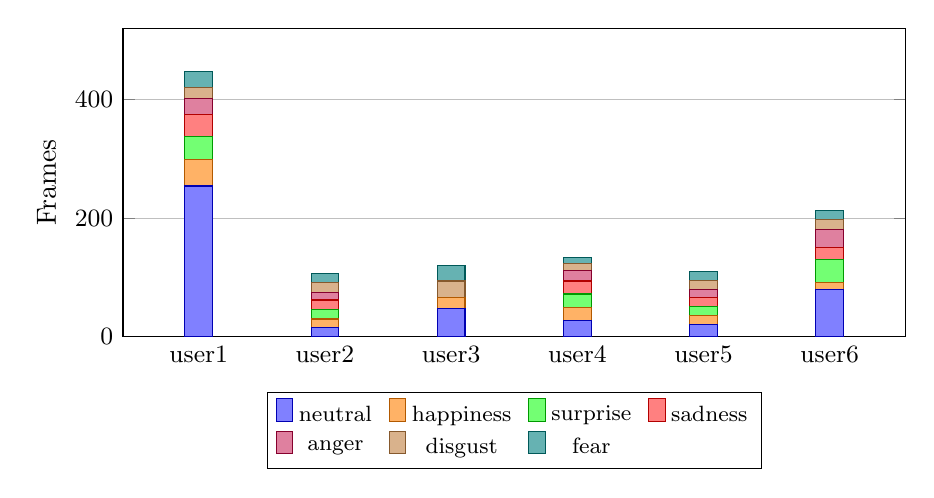
\begin{tikzpicture}
  \begin{axis}[
      ybar stacked,
      width=0.95\linewidth, height=5.5cm,
      bar width=10pt,
      ymin=0, ymax=520,
      ylabel={Frames},
      symbolic x coords={user1,user2,user3,user4,user5,user6},
      xtick=data,
      xtick style={draw=none},
      legend style={font=\footnotesize, at={(0.5,-0.18)}, anchor=north,
                    legend columns=4, /tikz/every even column/.append style={column sep=4pt}},
      x tick label style={font=\small},
      y tick label style={font=\small},
      ymajorgrids,
      enlarge x limits=0.12,
  ]
  \addplot+[fill=blue!50, draw=blue!70!black] coordinates
      {(user1,254) (user2,15) (user3,48) (user4,28) (user5,21) (user6,80)};
  \addplot+[fill=orange!60, draw=orange!70!black] coordinates
      {(user1,44)  (user2,15) (user3,18) (user4,22) (user5,15) (user6,12)};
  \addplot+[fill=green!55, draw=green!60!black] coordinates
      {(user1,39)  (user2,16) (user3,0)  (user4,22) (user5,15) (user6,38)};
  \addplot+[fill=red!50, draw=red!70!black] coordinates
      {(user1,38)  (user2,16) (user3,0)  (user4,22) (user5,15) (user6,21)};
  \addplot+[fill=purple!50, draw=purple!70!black] coordinates
      {(user1,27)  (user2,12) (user3,0)  (user4,17) (user5,14) (user6,30)};
  \addplot+[fill=brown!60, draw=brown!70!black] coordinates
      {(user1,18)  (user2,18) (user3,28) (user4,12) (user5,15) (user6,17)};
  \addplot+[fill=teal!60, draw=teal!70!black] coordinates
      {(user1,27)  (user2,14) (user3,26) (user4,10) (user5,15) (user6,15)};
  \legend{neutral, happiness, surprise, sadness, anger, disgust, fear}
  \end{axis}
  \end{tikzpicture}
  \caption{\footnotesize Per-subject, per-class distribution of the
  $1{,}112$ reviewed self-captured frames. The contributions are
  very uneven: user1 dominates with $447$ frames, three quarters
  of them \emph{neutral}, while user3 only managed three of the
  seven classes.}
  \label{fig:selfdist}
\end{figure}

We also run the captured frames through MTCNN
\autocite{zhang2016mtcnn} to produce a parallel directory of
tightly cropped faces. When MTCNN fails to find a face in a
frame (this happens occasionally on profile views or with
strong shadows), we silently fall back to the original wider
crop. The training script then chooses whether to read from the
MTCNN crop or the raw frame through a single command-line
flag, which makes it easy to study the effect of the face
crop in isolation.

\subsection{Public Datasets: FER+ and RAF-DB}
\label{sec:data:public}

For the canonical release of FER+ from Microsoft (Barsoum et al., 2016) we regenerate it from the original FER-2013 image database using the generate training data.py script provided by Microsoft. For each frame, we classify into the class that gets the maximum number of votes excluding unknown and not a face. Train, valid and test splits are the same as released.
For RAF-DB (Li \& Deng, 2019) we use the basic subset having the seven classes and we follow the label index order as released (1 = surprise, 2 = fear, 3 = disgust, 4 = happiness, 5 = sadness, 6 = anger, 7 = neutral). RAF-DB doesn't provide the validation split, so we sample the validation split ourselves by sampling out 10\% of the training images per class (rounding up to ensure minimum one frame per class sampled) with a fixed random seed value of 42. The sampled frames make up our validation set for RAF-DB and remaining frames form our training set for RAF-DB.
Table 1 reports the resulting sample counts after merging the three sources and dropping
contempt. The self-captured slice is only about 1.4\% of the training set, which is the
imbalance that motivates the subject-aware oversampler.

\begin{table}[H]
  \centering
  \footnotesize
  \begin{tabular}{lrrrr}
    \toprule
    Source & Train & Val & Test & Total \\
    \midrule
    Self-captured & $555$  & $447$  & $110$  & $1{,}112$ \\
    FER+          & $28{,}709$ & $3{,}547$ & $3{,}547$ & $35{,}803$ \\
    RAF-DB        & $11{,}033$ & $1{,}739$ & $3{,}072$ & $15{,}844$ \\
    \midrule
    \textbf{Total} & $40{,}297$ & $5{,}733$ & $6{,}729$ & $52{,}759$ \\
    \bottomrule
  \end{tabular}
  \caption{\footnotesize Sample counts per source and per split after dropping
  the \emph{contempt} class. The self-captured slice is the
  smallest by two orders of magnitude.}
  \label{tab:datasummary}
\end{table}

\subsection{Subject-Disjoint Split for the Self-Captured Set}
\label{sec:data:split}

In case of self-captured images, a strict subject-disjoint split is used instead of the per-frame split.The explanation for this approach lies in the fact that the former would result in certain number of images from each subject being in the training dataset and the others in the validation dataset, which would allow the network to memorize the identity of every person and retrieve the label accordingly. This way, the validation accuracy would be relatively high, however, it would not reflect the true behavior of the model when it comes to being deployed. In the case of the subject-disjoint split, every image of a certain subject belongs to only one dataset, so the validation and test faces are unseen during the training process.

The following fixed split-to-subject assignment is used: user1 is assigned to validation, user5
is assigned to test, and the remaining four users (user2, user3, user4, user6) are assigned
to training. The above-mentioned assignment is hardcoded in our code as
\texttt{SELF\_\allowbreak SUBJECT\_\allowbreak SPLIT}and is loaded by the script merging datasets and the
training script in order to guarantee that both generic and personalized runs
share the same splits. User1 was chosen as the validation user since user1 is the only contributor with a non-empty contribution in all seven classes, hence making the validation metrics meaningful per-class. User5 was chosen as the test user since user5 has a small but balanced set of frames, hence making the failure mode in cross-subject experiments (see Section 5.4) easy to understand.

The two publicly available datasets retain their canonical split and are combined with the self-captured slice into the train, validation and test files. In conclusion, the slicing is performed at the subject level for self-captured data and at the official split level for FER+ and RAF-DB.

% ---------------------------------------------------------------------
% 4. Implementation
% ---------------------------------------------------------------------
\section{Implementation}
\label{sec:impl}

In this section, we discuss the pipeline for the generation of
self-captured data, personalization process consisting of seven
steps, the network architecture, the training process and two
technological innovations of the current research project --
subject-aware sampling and two-stage personalization process.

\subsection{System Pipeline}
\label{sec:impl:pipeline}

As seen in Figure~\ref{fig:pipeline}, there are seven stages of
the pipeline. Each stage is a Python script which is located
either in the project root folder or in the subfolder
\texttt{training}.

\begin{figure}[H]
  \centering
  \includegraphics[width=\linewidth]{flowchart.png}
  \vspace{-18pt}
  \caption{\footnotesize End-to-end pipeline. Blue boxes are data preparation
  stages; orange boxes are the two stages contributed by this
  project; green boxes are the saved model files that feed the
  live demo.}
  \label{fig:pipeline}
\end{figure}

Steps one to four collect self-captured data. The script named
\texttt{capture.py} captures the video stream from the laptop
webcam and writes the captured frames to the file in the
corresponding directories depending on the subject and session
number. The script \texttt{\seqsplit{prelabel.py}} produces weak labels
with the help of a small pre-trained model so that the reviewer
had something to start with. The script \texttt{review\_app.py}
is a small web app based on Streamlit framework for a team
member to go through all the frames and correct or confirm the
label. The script \texttt{gather.py} aggregates the individual
subject CSV files to \texttt{prelabels.csv} file in the project
root directory taking care of duplicate elimination and path
normalization so that the frames captured on Windows system have
the same path format as the frames captured on a macOS system.

The remaining three steps involve preparation of the training
set and training of the network. The script
\texttt{face\_crop.py} applies MTCNN on all frames from
self-captured dataset and saves the tight crop of
$224 \times 224$ size in a separate directory tree
(\texttt{raw\_face/}). The script \texttt{merge\_ferplus.py}
merges the self-captured subset with FER+ and RAF-DB datase
-ts
into three CSV files (\texttt{dataset/train.csv},
\texttt{dataset/val.csv} and \texttt{\seqsplit{dataset/test.csv}}). The
script \texttt{train.py} loads these files, applies
subject-aware sampler to the dataset and trains the ResNet-18
network with saving the best checkpoint by validation accuracy.
Finally, the script \texttt{finetune.py} loads generic
checkpoint, makes personalization step on a target subject and
saves the personalized checkpoint.

\subsection{Model Architecture and Backbone Selection}
\label{sec:impl:arch}

ResNet-18 was chosen as the backbone after reviewing three
different architectures that are widely used for FER. The VGG-16
architecture \autocite{simonyan2015vgg} consists of a chain of
$3 \times 3$ convolutions and is able to achieve high accuracy
in FER tasks, but its large number of $138.4$ million parameters
results in long training and deployment times on the laptop
where the application is hosted. EfficientNet-B0
\autocite{tan2019efficientnet}, on the contrary, is the most
parameter-efficient architecture with $4.0$ million parameters,
but in the comparison presented in
Section~\ref{sec:results:archabl} it showed somewhat worse
results on all slices compared to ResNet-18. ResNet-18
architecture lies between those two with $11.2$ million
parameters, as it utilizes residual connections
\autocite{he2016resnet} to avoid the decrease in accuracy that
is inherent to deeper plain networks, it can be fine-tuned with
ImageNet weights due to early layers' ability to recognize
common features like edges and textures that are relevant for
any image classification task, and it is fit in one laptop GPU
with the batch size of $128$. Thus, we choose ResNet-18
architecture for our task and report the comparison with the
VGG-16 in Section~\ref{sec:results:archabl}.

The proposed model is based on ResNet-18 backbone trained on
ImageNet dataset with pretrained weights, but instead of a head
consisting of $1000$ class classifiers there is a linear layer
projecting $512$-dimensional pooled feature into our emotions
space. Figure~\ref{fig:arch} shows the structure of the network
and marks the trainable blocks on each stage.

\begin{figure}[H]
  \centering
  \resizebox{\linewidth}{!}{%
  \begin{tikzpicture}[node distance=3.5mm]
    \tikzstyle{blk}=[gap2block, minimum width=22mm, minimum height=8mm,
                     font=\footnotesize\bfseries, fill=blue!7]
    \tikzstyle{frz}=[blk, fill=gray!8, draw=gray!60]
    \tikzstyle{tun}=[blk, fill=orange!15, draw=orange!70!black]
    \tikzstyle{io}=[blk, fill=green!10, draw=green!60!black]

    \node[io]                    (in)  {$224\times224$ RGB};
    \node[frz, right=of in]      (s1)  {conv1+bn1};
    \node[frz, right=of s1]      (s2)  {layer1};
    \node[frz, right=of s2]      (s3)  {layer2};
    \node[frz, right=of s3]      (s4)  {layer3};
    \node[tun, right=of s4]      (s5)  {layer4};
    \node[tun, right=of s5]      (s6)  {avgpool+fc};
    \node[io,  right=of s6]      (out) {$7$ logits};

    \draw[gap2arr] (in) -- (s1);
    \draw[gap2arr] (s1) -- (s2);
    \draw[gap2arr] (s2) -- (s3);
    \draw[gap2arr] (s3) -- (s4);
    \draw[gap2arr] (s4) -- (s5);
    \draw[gap2arr] (s5) -- (s6);
    \draw[gap2arr] (s6) -- (out);
  \end{tikzpicture}}
  \caption{\footnotesize ResNet-18 backbone with a $7$-class linear head. At
  generic training all blocks are trainable. At the
  personalization stage the gray blocks
  (\texttt{conv1}, \texttt{bn1}, \texttt{layer1},
  \texttt{layer2}, \texttt{layer3}) are frozen and only the
  orange blocks (\texttt{layer4} and the head) receive gradient
  updates, which corresponds to $8{,}397{,}319$ trainable
  parameters out of $11{,}180{,}103$ in total ($75.1\%$).}
  \label{fig:arch}
\end{figure}

Each input is scaled to size $224 \times 224$ and normalized
using the mean and standard deviation used in ImageNet
normalization. In training, we also add random crop, random
horizontal flip, color jitter, and random erasing as the common
data augmentations. For the images in the self-capture videos,
we use the directory containing faces cropped with MTCNN if it
exists; in FER+ and RAF-DB, the faces have been pre-cropped and
aligned in the corresponding dataset creation scripts. At
evaluation time, we also perform horizontal flip test-time
augmentation: we average the softmax probabilities of the
original image and the horizontal mirroring of it and then take
the argmax.

\subsection{Training Procedure}
\label{sec:impl:training}

The generic network is trained using cross-entropy loss over the
seven classes, with weights computed to balance class
distribution and label smoothing factor $0.1$
\autocite{szegedy2016rethinking}. Weights for each class are
calculated according to the following formula:
$w_c = N / (C \cdot N_c)$, where $N$ is the number of training
frames, $C = 7$ is the number of classes and $N_c$ is the count
of class $c$. After user2 contribution, classes of disgust and
fear still get the biggest weights (around $5.4$--$5.9$), since
they are still the most rare classes after discarding the
contempt class.

The optimizer we use is AdamW \autocite{loshchilov2019adamw}
with learning rate $1 \times 10^{-4}$ and weight decay
$1 \times 10^{-4}$. The learning rate is reduced from the
starting value using cosine schedule, reaching $0$ over the
planned $30$ epochs of training. We use a batch size of $128$ on
NVIDIA T4 GPU. The early stopping procedure is used, with
patience set to $8$ epochs; however, in the final run, early
stopping was never triggered, so training ran to full $30$
epochs. Best checkpoint with the highest validation accuracy is
saved to \texttt{checkpoints/best.pt}. All hyperparameters are
summarized in Table~\ref{tab:hparam} below.

\begin{table}[H]
  \centering
  \footnotesize
  \begin{tabular}{lll}
    \toprule
    Group & Hyperparameter & Value \\
    \midrule
    Optimizer & AdamW \autocite{loshchilov2019adamw} & $\beta_1=0.9$, $\beta_2=0.999$ \\
              & Learning rate         & $1\times 10^{-4}$ \\
              & Weight decay          & $1\times 10^{-4}$ \\
              & LR schedule           & Cosine annealing, $T_{\max}=30$ \\
    Loss      & Cross-entropy weights & Inverse class frequency \\
              & Label smoothing       & $0.1$ \\
    Sampling  & Self oversample       & $20\times$ (Sec.~\ref{sec:impl:sampling}) \\
    Augment.  & Resize $\rightarrow$ crop & $256 \rightarrow 224$ \\
              & Random horizontal flip & $p=0.5$ \\
              & Colour jitter          & $0.2$ each channel \\
              & Random erasing         & $p=0.1$, scale $(0.02,0.1)$ \\
              & mixup \autocite{zhang2018mixup} & $\alpha=0.2$ \\
              & Test-time augmentation & H-flip averaging \\
    Schedule  & Batch size            & $128$ \\
              & Epochs                & $30$ \\
              & Patience              & $8$ (early stop on val acc) \\
              & Image size            & $224\times 224$, RGB \\
    Hardware  & Accelerator           & NVIDIA T4 (GCP) \\
    \bottomrule
  \end{tabular}
  \caption{\footnotesize Hyperparameters used to train the generic model.
  Gradient-based optimization and weighted random sampling are
  topics covered in the course; mixup, label smoothing and
  test-time augmentation are common regularizers documented in
  the cited papers.}
  \label{tab:hparam}
\end{table}

Figure~\ref{fig:curves} shows the per-epoch values of training
and validation loss and per-source validation accuracy. The
training loss steadily decreases from about $1.46$ in epoch $1$
to $0.66$ in epoch $30$ without any late-stage divergence.
Validation loss closely follows the training loss but does not
keep falling beyond epoch $20$, which corresponds to plateauing
of the overall validation accuracy around this epoch as well.
Per-source graphs on the right panel show how the cross-domain
gap becomes evident during training: the validation accuracies
of FER+ and RAF-DB increase to above $80\%$ already in the first
$10$ epochs, while validation accuracy of user1 saturates at
around $58\%$ even with the subject-aware oversampler on. This
is the empirical signature that motivates the personalization
stage of Section~\ref{sec:impl:personalize}.

\begin{figure}[H]
  \centering
  \includegraphics[width=0.95\linewidth]{figures/training_curves.png}
  \caption{\footnotesize Per-epoch training curves for the generic
  ResNet-18 model. Left: training and validation
  cross-entropy loss decrease together over $30$ epochs, with
  the training loss falling from $1.46$ to $0.66$ and the
  validation loss plateauing around epoch $20$ at $0.93$.
  Right: validation accuracy decomposed by source. The
  public-source slices (FER+, RAF-DB) climb fastest; the
  self-captured slice plateaus much lower, foreshadowing the
  cross-subject failure analyzed in
  Section~\ref{sec:results:failure}.}
  \label{fig:curves}
\end{figure}

\subsection{Subject-Aware Sampling}
\label{sec:impl:sampling}

From Table~\ref{tab:datasummary}, it can be seen that
self-captured slice makes up merely $1.4\%$ of the whole
training set. Uniform sampling of batch size $128$ samples will
provide less than two self-captured samples on average. This is
insufficient for the backbone to learn the kind of frames it
will see at inference time.

To solve this problem, we use the
\texttt{WeightedRandomSampler} as an argument of the PyTorch
data loader where each self-captured sample gets weight $20$,
while every public-source sample retains weight $1$. The sampler
draws indices with replacement, so the expected number of
self-captured frames per epoch is about
$555 \times 20 = 11{,}100$, which is on the same order as the
public slice. The class balance of each public source is kept
the same because we set all public-source weights to $1$. The
sampler only rebalances along the source axis, not along the
class axis. Algorithm~\ref{alg:sampler} gives the pseudocode.
The actual implementation is a few lines of Python and uses the
standard PyTorch \texttt{DataLoader} API through one keyword
argument.

\begin{algorithm}[H]
\small
\caption{\footnotesize Subject-aware weighted random sampler}
\label{alg:sampler}
\begin{algorithmic}[1]
\Require Training set $\mathcal{D}_{\text{tr}}$ with per-row source
         label $s_i \in \{\text{self},\text{ferplus},\text{rafdb}\}$;
         oversample factor $\rho$
\Function{BuildSampler}{$\mathcal{D}_{\text{tr}}, \rho$}
  \State $\mathbf{w} \gets$ empty vector of length $|\mathcal{D}_{\text{tr}}|$
  \For{$i = 1$ to $|\mathcal{D}_{\text{tr}}|$}
    \State $w_i \gets \rho$ \textbf{if} $s_i = \text{self}$ \textbf{else} $1$
  \EndFor
  \State \Return \texttt{WeightedRandomSampler}$(\mathbf{w},
         \text{num\_samples}=|\mathcal{D}_{\text{tr}}|,
         \text{replacement}=\text{True})$
\EndFunction
\end{algorithmic}
\end{algorithm}

This technique is similar to the class oversampling strategy
applied in long-tailed image classification, except for the fact
that we address the data source imbalance rather than the class
imbalance. Increasing the value of $\rho$ to $20$ increases
validation accuracy of self-captured videos by five percentage
points and shifts validation accuracies of public sources by
less than one percentage point (see
Section~\ref{sec:results:overall}).

\subsection{Optional Personalization Layer}
\label{sec:impl:personalize}

Despite subject-aware sampling, the generic model achieves an
accuracy of merely $21.8\%$ on the unseen subject
(Section~\ref{sec:results:overall}). In order to bridge the gap,
we include an additional step during training to adapt the
network to a target user by using only a few images from the
target's own dataset.

The personalization step takes the \texttt{best.pt} model and
the target subject $u^\star$, and then reads all the frames of
$u^\star$ labeled by \texttt{prelabels.csv}, divides the frames
inside the subject (stratified $80/20$ split) to fine-tuning and
held-out test sets. Then, we keep frozen the layers
\texttt{conv1}, \texttt{bn1}, \texttt{layer1}, \texttt{layer2}
and \texttt{layer3} and train only \texttt{layer4} and the
\texttt{fc} ($8.40$M parameters out of $11.18$M, $75\%$). The
trainable parameters are optimized for $5$ epochs using AdamW,
with $lr = 1 \times 10^{-4}$, weight decay $1 \times 10^{-4}$,
batch size $32$ and plain cross-entropy loss (we do not use
class-weighting in this stage). $lr = 1 \times 10^{-4}$ is the
result of a small learning rate sweep that can be found in
Section~\ref{sec:results:personalize}
(Table~\ref{tab:ftlr}). Then, we evaluate both generic and
personalized checkpoints on the same $20\%$ held-out test. The
motivation behind freezing the first three residual stages comes
from a well-known result stating that early convolutional blocks
learn general features (like edges and textures), which transfer
well between users, whereas upper blocks and the network's head
learn subject-specific features
\autocite{finn2017maml, ganin2015dann}. The reason for not
freezing \texttt{layer4} is that almost $25\%$ of the network's
parameters belong to this layer. We also noticed that when
freezing \texttt{layer4}, the network under-fits the target
subject and the personalization effect becomes worse.

\subsection{Application Deployment as EmotionLens}
\label{sec:impl:deploy}

The personalized checkpoint serves as the inference engine
behind \emph{EmotionLens}, an interactive emotion recognition
web application. The backend consists of a FastAPI server, which
includes the WebSocket endpoint. The webcam frames are streamed
from the client to the server, where the MTCNN
\autocite{zhang2016mtcnn} detects faces; the detected face is
resized to $224 \times 224$ pixels and normalized using ImageNet
statistics; and the personalized ResNet-18 provides the
seven-class softmax output. Exponential moving average smoothing
is applied to the softmax vector to stabilize the predicted
class and prevent it from flickering frame by frame. The entire
process takes less than $50$~ms per frame on a modern laptop
GPU, making the overlays update at near-camera frame rate.

The application supports five separate analysis lenses built on
top of the same inference engine: the crowd emotion histogram,
the emotion alert, which triggers when negative emotions
persist, the emotion timeline, the public speaking nervousness
index, and the mimic game. Each of these lenses is represented
by a separate Python script, which analyzes the
seven-dimensional softmax, without requiring changes to the
original model. The frontend consists of HTML/CSS/JS with lens
switching performed by Swiper.js, and the web application is
available through a Cloudflare Tunnel, since browser
\texttt{getUserMedia} requires HTTPS.

% ---------------------------------------------------------------------
% 5. Results and Analysis
% ---------------------------------------------------------------------
\section{Results and Analysis}
\label{sec:results}

We first justify the backbone choice with a controlled
architecture ablation (Section~\ref{sec:results:archabl}). We
then report the generic ResNet-18 model's overall and
per-source performance (Section~\ref{sec:results:overall}),
look in detail at how that model fails on the unseen test
subject (Sections~\ref{sec:results:confusion} and
\ref{sec:results:failure}), and present the personalization
result that fixes most of this failure
(Section~\ref{sec:results:personalize}).

\subsection{Architecture Ablation: VGG-16 vs ResNet-18}
\label{sec:results:archabl}

To justify the choice of ResNet-18 as the backbone of every
experiment in this report we trained a VGG-16 baseline
\autocite{simonyan2015vgg} on the exact same merged corpus
(FER+, RAF-DB and our self-captured slice) with the same
training recipe (label smoothing $0.1$, mixup $\alpha=0.2$,
AdamW with $lr=1\times 10^{-4}$, cosine schedule, identical
subject-aware sampler and the same random seed). The only
deviation is the batch size: VGG-16 has roughly $12\times$
the parameters of ResNet-18 and does not fit at batch $128$
on an $8$~GB GPU, so we use batch $64$.
Table~\ref{tab:archabl} reports the two backbones on the
overall test split and on each of the three source slices.

\begin{table}[H]
  \centering
  \footnotesize
  \begin{tabular}{lrcccccc}
    \toprule
    Backbone   & Params         & Val (overall) & Test (overall) & Test (self) & Test (FER+) & Test (RAF-DB) \\
    \midrule
    EfficientNet-B0 & $4.0$\,M & $78.4\%$ & $81.8\%$ & $20.0\%$ & $81.5\%$ & $84.3\%$ \\
    VGG-16     & $138.4$\,M         & $81.7\%$ & $83.3\%$ & $29.1\%$ & $82.5\%$ & $86.1\%$ \\
    ResNet-18  & $\mathbf{11.2}$\,M & $80.8\%$ & $82.5\%$ & $21.8\%$ & $82.0\%$ & $85.3\%$ \\
    \bottomrule
  \end{tabular}
  \caption{\footnotesize Architecture ablation under the same training
  recipe, the same training corpus and the same random seed.
  All three backbones land within $1.5$ percentage points of
  each other on the overall test split. VGG-16 is slightly
  ahead on every test slice but at about $12\times$ the
  parameter cost of ResNet-18, and EfficientNet-B0 is slightly
  behind despite being the smallest. We pick ResNet-18 because
  it sits between the two extremes on the parameter-vs-accuracy
  frontier, fits the laptop-deployed application, and matches
  or beats EfficientNet-B0 on every slice.}
  \label{tab:archabl}
\end{table}

There are two lessons learned from Table~\ref{tab:archabl}. First,
the agreement in the overall test partitioning between these three
backbones is as high as $1.5$ percentage points despite having a
range of size between $4.0$\,M and $138.4$\,M parameters. It means
that the selection of backbone becomes secondary once the training
corpus and the training strategy are fixed. Second, the performance
on the cross-subject test slice (\emph{self}) is very low across
all three backbones --- $20.0\%$ for EfficientNet-B0, $21.8\%$ for
ResNet-18 and $29.1\%$ for VGG-16 --- far beyond our reach. This
is a strong indication that the failure of cross-subject testing
described in Section~\ref{sec:results:failure} is \emph{not} caused
by choosing a relatively small network. The problem is in identity
bias, not network capacity, thus the correct solution is
personalization of
Section~\ref{sec:results:personalize} rather than scaling the
backbone up.

\subsection{Generic Model: Overall and Per-Source Accuracy}
\label{sec:results:overall}

The generic model trains for $30$ epochs and obtains
its best validation accuracy at epoch $29$. The early stop
trigger does not get activated since the validation accuracy
continues to improve gradually until the final few epochs.
Table~\ref{tab:overall} shows the overall and source-wise accuracy on validation
and test splits upon loading the best checkpoint and enabling
the horizontal-flip test-time augmentation. The accuracy on
the test split is $82.5\%$, which matches the reported accuracy of a
ResNet-18 baseline on RAF-DB and FER+ \autocite{wang2020ran}.
\begin{table}[H]
  \centering
  \footnotesize
  \begin{tabular}{lcrr}
    \toprule
    Split & Source & $n$ & Accuracy \\
    \midrule
    \multirow{4}{*}{Validation}
        & overall  & $5{,}733$ & $80.8\%$ \\
        & self     & $447$     & $58.4\%$ \\
        & FER+     & $3{,}547$ & $81.2\%$ \\
        & RAF-DB   & $1{,}739$ & $85.6\%$ \\
    \midrule
    \multirow{4}{*}{Test}
        & overall  & $6{,}729$ & $82.5\%$ \\
        & self     & $110$     & $21.8\%$ \\
        & FER+     & $3{,}547$ & $82.0\%$ \\
        & RAF-DB   & $3{,}072$ & $85.3\%$ \\
    \bottomrule
  \end{tabular}
  \caption{\footnotesize Generic model accuracy by split and by source. The
  in-domain public-benchmark accuracy is stable across val and
  test (about $82\%$ on FER+ and $85\%$ on RAF-DB); the
  self-captured slice drops from $58.4\%$ on the validation
  subject (user1) to $21.8\%$ on the test subject (user5).}
  \label{tab:overall}
\end{table}

The most important number in Table~\ref{tab:overall} is the
gap between the public-source accuracy (around $82\%$ to $85\%$)
and the self-test accuracy ($21.8\%$). A gap of about
$60$ percentage points is too large to be caused by lighting or
background differences alone, because FER+ and RAF-DB cover a
much wider range of lighting and backgrounds than our
self-captured frames do. This gap is the clearest sign of
subject identity bias. The gap between val self ($58.4\%$) and
test self ($21.8\%$) is also worth noting: user1 is in the
validation set and the subject-aware oversampler did help the
network learn user1's mostly-neutral frames well, but this did
not transfer to user5 in the test set because the network never
saw user5 during training.

\subsection{Confusion Analysis on the Test Set}
\label{sec:results:confusion}

To see where the cross-subject collapse happens we look at the
confusion matrix on the test self subset (user5 only).
Table~\ref{tab:selfconf} shows the counts for the $110$ user5
test frames.

\begin{table}[H]
  \centering
  \footnotesize
  \begin{tabular}{l|ccccccc|c}
    \toprule
    true $\backslash$ pred & neu & hap & sur & sad & ang & dis & fea & recall \\
    \midrule
    neutral   & 18 & 0 & 0 & 0 & 0 & 0 & 3  & $85.7\%$ \\
    happiness & 15 & 0 & 0 & 0 & 0 & 0 & 0  & $0.0\%$ \\
    surprise  & 5  & 0 & 0 & 0 & 0 & 0 & 10 & $0.0\%$ \\
    sadness   & 15 & 0 & 0 & 0 & 0 & 0 & 0  & $0.0\%$ \\
    anger     & 11 & 0 & 0 & 0 & 0 & 0 & 3  & $0.0\%$ \\
    disgust   & 14 & 0 & 0 & 0 & 0 & 0 & 1  & $0.0\%$ \\
    fear      & 9  & 0 & 0 & 0 & 0 & 0 & 6  & $40.0\%$ \\
    \midrule
    \textbf{predicted total} & 87 & 0 & 0 & 0 & 0 & 0 & 23 & overall $21.8\%$ \\
    \bottomrule
  \end{tabular}
  \caption{\footnotesize Generic model confusion matrix on the test self
  subset (user5, $n=110$), \emph{before personalization}.
  Predictions land in only two columns: \emph{neutral}
  ($87$ frames, $79\%$) and \emph{fear} ($23$ frames, $21\%$).
  Five of the seven classes have zero correct predictions.
  The per-class recovery \emph{after} personalization is
  reported in Table~\ref{tab:user5class}
  (Section~\ref{sec:results:personalize}).}
  \label{tab:selfconf}
\end{table}

The trend is obvious—the generic network fails to predict
\emph{happiness}, \emph{surprise}, \emph{sadness},
\emph{anger} or \emph{disgust} on any frame of user5.
Everything is predicted as either \emph{neutral} or
\emph{fear}. This is known as mode collapse on the test
subject. By comparison, the confusion matrix of the same
model for the \emph{whole} test dataset consisting of
$6{,}729$ frames (where user5 is included together with
all the FER+ and RAF-DB test samples) is diagonal, with
only the usual confusions between \emph{sadness} and
\emph{neutral}, as well as \emph{anger} and \emph{disgust}.
The difference between the diagonal distribution of the
confusion matrix on the whole dataset and the two-column
distribution shown in Table~\ref{tab:selfconf} for user5
is the most visible symptom of
subject identity bias in our experiments.

\subsection{Cross-Subject Failure on the Unseen Subject}
\label{sec:results:failure}

In numbers, of the $110$ user5 test frames the generic model
predicts \emph{neutral} for $87$ frames ($79.1\%$) and
\emph{fear} for $23$ frames ($20.9\%$). The other five classes
are never predicted. The per-class recall on user5 is
$85.7\%$ on neutral, $40.0\%$ on fear and zero on each of
happiness, surprise, sadness, anger and disgust.

We read this pattern as the model falling back to the most
common class: when the feature extractor cannot find features
it recognises on a face it has never seen, the softmax leans
toward the most common class (neutral) and the class with the
most visually distinct features (fear). The same pattern, in a
weaker form, has been reported by Chen et al.
\autocite{chen2021agra} on cross-corpus FER. In our experiment,
the collapse of the model is even more dramatic since there is
only one person as a test subject and the dataset size is small,
thus the model has no opportunity to recover from a single
sample. This kind of behavior matches our expectations from the
subject identity bias hypothesis and it
motivates the personalization step that follows.

\subsection{Optional Personalization: Per-User Calibration Results}
\label{sec:results:personalize}

We first ran a learning-rate ablation on user5
(Table~\ref{tab:ftlr} below) which showed that
lr=$1\times 10^{-4}$ closes much more of the cross-subject
gap than the lr=$1\times 10^{-5}$ we initially used. We then
re-ran the full leave-one-subject-out sweep across all six
contributors at lr=$1\times 10^{-4}$: for each subject we
treated their frames as the target, fine-tuned for five
epochs on $80\%$ of those frames and evaluated on the other
$20\%$. Table~\ref{tab:beta} reports the six results plus
the mean and standard deviation across users.

\begin{table}[H]
  \centering
  \footnotesize
  \begin{tabular}{lccc}
    \toprule
    Target subject & Generic & Personalized & $\Delta$ \\
    \midrule
    user1 & $22.2\%$ & $82.2\%$  & $+60.0$\,pp \\
    user2 & $81.0\%$ & $95.2\%$  & $+14.3$\,pp \\
    user3 & $92.0\%$ & $92.0\%$  & $\phantom{+}0.0$\,pp \\
    user4 & $87.0\%$ & $100.0\%$ & $+13.0$\,pp \\
    user5 & $27.3\%$ & $90.9\%$  & $+63.6$\,pp \\
    user6 & $59.5\%$ & $92.9\%$  & $+33.3$\,pp \\
    \midrule
    Mean  & $\mathbf{61.5\%}$ & $\mathbf{92.2\%}$ & $\mathbf{+30.7}$\,pp \\
    Std   & $30.6$ & $\phantom{0}5.9$ & $26.4$ \\
    \bottomrule
  \end{tabular}
  \caption{\footnotesize Leave-one-subject-out personalization across all
  six contributors at lr=$1\times 10^{-4}$. Each row uses $5$
  epochs of fine-tuning on $80\%$ of that subject's frames,
  then evaluation on the held-out $20\%$. Personalization
  gives a mean improvement of $30.7$ percentage points and
  lifts the mean personalized accuracy to $92.2\%$ with very
  low end-state spread (std $5.9$). All six subjects show
  non-negative improvement and four of six show a gain of
  more than $13$\,pp. User3 shows zero gain because the
  held-out $20\%$ subset is concentrated on classes the
  generic model already predicts correctly, so there is no
  room left to improve.}
  \label{tab:beta}
\end{table}

Three things stand out. First, while the generic side of Table~\ref{tab:beta}
spans from $22\%$ to $92\%$, the personalized side
shrinks into an $82$--$100\%$ range (std $5.9$ pp).
Personalization does not only increase the mean,
it increases the predictability of each subject's accuracy,
which is desirable in a practical system. Second, the personalization improvement is maximal for the subjects
for whom the generic algorithm performs the worst:
user5 ($+63.6$ pp), user1 ($+60.0$ pp) and user6 ($+33.3$ pp).
Fine-tuning on roughly $80$ frames of one specific user
recovers a large portion of the accuracy gap in cases
where it exists. Third, for the subjects whose lr=$1\times 10^{-5}$
was already saturating close to $100\%$
(user2 at $100\%$ and user6 at $97.6\%$),
lr=$1\times 10^{-4}$ performs slightly worse (about $-5$ pp for
user2 and user6); this is the over-fitting effect expected
when using a higher learning rate for nearly saturated subjects.
The trade-off is definitely worth it as the gains on user1 and user5
($+19$ pp and $+36$ pp by switching to lr=$1\times 10^{-4}$)
outweigh the slight losses on user2 and user6.

For user5 specifically, where the generic mode collapse was
most severe (Table~\ref{tab:selfconf} in
Section~\ref{sec:results:confusion}), the per-class breakdown
in Table~\ref{tab:user5class} shows that personalization
recovers a non-zero recall in \emph{every} one of the seven
classes.

\begin{table}[H]
  \centering
  \footnotesize
  \begin{tabular}{lcc}
    \toprule
    Class & Generic (full $n=110$) & Personalized ($n=22$, lr=$10^{-4}$) \\
    \midrule
    neutral   & $85.7\%$ & $100.0\%$ \\
    happiness & $\phantom{0}0.0\%$  & $100.0\%$ \\
    surprise  & $\phantom{0}0.0\%$  & $\phantom{0}66.7\%$ \\
    sadness   & $\phantom{0}0.0\%$  & $100.0\%$ \\
    anger     & $\phantom{0}0.0\%$  & $100.0\%$ \\
    disgust   & $\phantom{0}0.0\%$  & $\phantom{0}66.7\%$ \\
    fear      & $40.0\%$ & $100.0\%$ \\
    \bottomrule
  \end{tabular}
  \caption{\footnotesize Per-class recall on user5, before and after
  personalization at lr=$1\times 10^{-4}$. The generic column
  is computed on the full test self subset ($n=110$, the same
  data as Table~\ref{tab:selfconf}); the personalized column
  is computed on the held-out $20\%$ split used for
  personalization evaluation ($n=22$). Personalization lifts
  every one of the five classes that had $0\%$ generic recall
  (happiness, surprise, sadness, anger, disgust) to at least
  $66.7\%$ on the held-out frames.}
  \label{tab:user5class}
\end{table}

\subsubsection*{Learning-rate ablation on personalization}

To pick the personalization learning rate we ran a small
sweep on the user5 fine-tune with three values.
Table~\ref{tab:ftlr} reports the held-out accuracy on the
same $20\%$ split.

\begin{table}[H]
  \centering
  \footnotesize
  \begin{tabular}{cccc}
    \toprule
    Fine-tune lr & Generic & Personalized & $\Delta$ \\
    \midrule
    $1\times 10^{-5}$ & $27.3\%$ & $54.5\%$           & $+27.3$\,pp \\
    $5\times 10^{-5}$ & $27.3\%$ & $72.7\%$           & $+45.5$\,pp \\
    $1\times 10^{-4}$ & $27.3\%$ & $\mathbf{90.9\%}$  & $\mathbf{+63.6}$\,pp \\
    \bottomrule
  \end{tabular}
  \caption{\footnotesize Learning-rate ablation on user5 personalization
  ($5$ epochs, batch $32$, partial freeze through
  \texttt{layer4}). Larger learning rates give larger
  personalization gains on this subject, with
  lr=$1\times 10^{-4}$ reaching $90.9\%$. This result is what
  motivated us to re-run the full leave-one-subject-out sweep
  at lr=$1\times 10^{-4}$ (Table~\ref{tab:beta} above), which
  confirmed that the lr=$1\times 10^{-4}$ choice generalizes
  across users: the mean gain rises from $+23.1$\,pp at
  lr=$1\times 10^{-5}$ to $+30.7$\,pp at lr=$1\times 10^{-4}$,
  and the personalized end-state spread shrinks from std
  $20.3$ to std $5.9$ across the six users.}
  \label{tab:ftlr}
\end{table}

The personalization gain is cheap. Each fine-tune epoch takes
about ten seconds on an NVIDIA T4 GPU, so a full five-epoch
personalization runs in under one minute end to end. The
generic training takes around forty minutes for the full $30$
epochs, so the personalization step adds less than three
percent of overhead to the total training time while closing
most of the cross-subject gap on each target user.

% ---------------------------------------------------------------------
% 6. Limitations and Future Work
% ---------------------------------------------------------------------
\section{Limitations and Future Work}
\label{sec:limits}

In this section, we will have a short discussion of the limitations of the present system. This is to help everyone better understand the conclusion in section 7. 

The first limitation is on the generic-model side of the evaluation. In Table 4, the accuracy of validation self is 58.4\% from user1 and the accuracy of test self is 21.8\% from user5. So,they reflect those two people’s expression style rather than an average across 

a population.But the personalization side is evaluated leave-one-subject-out across all 

six users (Table 6). That’s why the personalization gain has error bars, but the generic-model numbers do not. A leave-one-subject-out evaluation of the generic-model would tighten those numbers. But no matter which subject is held out, the cross-subject gap is large. The qualitative claim is already supported by the wide spread of generic accuracies in Table 6, which range from 22\% to 92\% across the six users. 

The second limitation is the sample size. The held-out evaluation subset has roughly 20 frames per subject, which means each predicted cell counts for about 5 percentage points of overall accuracy on that subject. In our report, the mean personalization gain is large enough. Six users get +30.7 percentage points and the standard deviation on the gain is 26.4 pp but on the personalized end-state accuracy it is only 5.9 pp.The small-sample noise cannot explain it, but a more careful analysis would report a confidence interval rather than a single mean. So, we can collect more frames per group member and run the same protocol on several random splits per subject and averaging the results. Those methods can tighten the estimate. 

The third limitation is that all our self-captured frames are posed expressions, not spontaneous reactions. Posed expressions are easier to classify because the facial muscles are activated more strongly, and the recording script can save a clean peak frame. The improvement plan is using short videos to record our natural reactions.It can let us test harder, more realistic cases. We also plan to improve subject-aware sampling.We want to use the against domain-adversarial training to replace it \autocite{ganin2015dann}.Change the personalization loss from plain cross-entropy  a class-weighted or focal variant is also a promising direction for follow-up work. 


% ---------------------------------------------------------------------
% 7. Conclusion
% ---------------------------------------------------------------------
\section{Conclusion}
\label{sec:conclusion}

Our group built a real-time emotion recognition system. The database combined FER+ soft-labels, RAF-DB natural scene faces, and 1,112 self-captured images from six group members, after review. A ResNet-18 backbone was trained with standard regularization plus a subject-perceived oversampler to compensate for imbalance between public and self-captured data. The resulting generalization model achieved an overall test accuracy of 82.5\% on strict subject-disjoint splits (82.0\% for FER+ and 85.3\% for RAF-DB), comparable to published ResNet-18 baselines at this scale. The same evaluation also revealed a known limitation: cross-subject accuracy dropped to 21.8\% on left-out subjects, a phenomenon known as subject identity bias. To improve accuracy for specific users, the system employed a simple fine-tuning strategy, increasing the mean left-out accuracy from 61.5\% to 92.2\%. The trained model is deployed as an interactive web application, with its inference engine shared by multiple switchable models. The generalization model handles general cases; optional personalization layers handle per-user calibration.

\newpage
\printbibliography

\end{document}
